\documentclass[12pt, a4paper]{article}

\usepackage[utf8]{inputenc}
\usepackage[T1]{fontenc}
\usepackage[russian]{babel}
\usepackage[oglav,spisok,boldsect,eqwhole,figwhole,hyperref,hyperprint,remarks,greekit]{./style/fn2kursstyle}
\usepackage{tikz}
\graphicspath{{./style/}{./figures/}}

\usepackage{multirow}
\usepackage{supertabular}
\usepackage{multicol}
\usepackage{mathtools}
% Параметры титульного листа
\title{Прямые методы решения систем
	линейных алгебраических уравнений}
\lab{1}
\author{И.\,Е.~Дыбко}
\creator{С.\,И.~Тихомиров}
\supervisor{А.\,О.~Гусев}
\group{ФН2-51Б}
\date{2024}

% Переопределение команды \vec, чтобы векторы печатались полужирным курсивом
\renewcommand{\vec}[1]{\text{\mathversion{bold}${#1}$}}%{\bi{#1}}
\newcommand\thh[1]{\text{\mathversion{bold}${#1}$}}
%Переопределение команды нумерации перечней: точки заменяются на скобки
\renewcommand{\labelenumi}{\theenumi)}
\begin{document}
	
	\maketitle
	
	\tableofcontents
	\section{Описание использованных алгоритмов}
	\section{Ответы на контрольные вопросы}
	
	\begin{enumerate}
	\item \textbf{Каковы условия применимости метода Гаусса без выбора
	и с выбором ведущего элемента?}
	
		\textbf{Без выбора ведущего элемента:} Метод Гаусса может быть применен, если на всех шагах на главной диагонали не возникает нулевых элементов: $$a^{(i-1)}_{ii}\ne 0, i = 1,2,\ldots,n.$$

		 \textbf {С выбором ведущего элемента:} Метод с выбором ведущего элемента  применим всегда, когда матрица невырожденная ($\det A \ne 0$).
		 
	\item \textbf{Докажите, что если $\det A \ne 0$, то при выборе главного
	элемента в столбце среди элементов, лежащих не выше главной диагонали, всегда найдется хотя бы один элемент, отличный от нуля.}
	
		 Для любой невырожденной матрицы обязательно существует хотя бы один ненулевой элемент в каждом столбце среди элементов, которые находятся на главной диагонали или ниже ее. В противном случае хотя бы один столбец состоял бы из нулей, что привело бы к нулевому определителю, что противоречит условию ($\det A \ne 0$):
	

	\item \textbf{В методе Гаусса с полным выбором ведущего элемента приходится не только переставлять уравнения, но и менять нумерацию неизвестных. Предложите алгоритм, позволяющий восстановить первоначальный порядок неизвестных.}
	
	Создадим два массива linearr и columnarr, где изначально будет числовая последованность $i=1,2,\ldots,n$. При перестановке уравнений (строк) или смене нумерации неизвестных (столбцов) будем менять элементы в этих массивах. 
	
	
	
	\item \textbf{Оцените количество арифметических операций, требуемых
	для QR-разложения произвольной матрицы $A$ размера $n \times n$.}
	\begin{enumerate}
		\item \textbf{ Метод Грамма--Шмидта}
		
		Проекция вектора на другой вектор требует $2n$ операций. Для каждого из $n$ столбцов вычисляется $n-1$ проекций. Таким образом, общее количество операций для метода Грамма-Шмидта составляет $O(n^3)$ .
		\item \textbf{ Метод отражений Хаусхолдера}
		
		Отражение Хаусхолдера для каждого столбца требует $2n^2$ операций, так как оно применяется ко всем элементам матрицы ниже диагонали. Поскольку для матрицы размером $n \times n$ таких отражений будет $n-1$, общая сложность метода составляет $O(n^3)$.
		\item \textbf{ Метод вращений Гивенса}
		
		Метод вращений Гивенса использует последовательные вращения для зануления элементов матрицы. Вращение затрагивает только два элемента одновременно, что делает метод особенно эффективным для разреженных матриц (сложность $O(n^2)$). Для плотных матриц, как правило, требуется также $O(n^3)$ операций, так как необходимо применять множество вращений ко всем элементам матрицы.
	\end{enumerate}



	\item \textbf{Что такое число обусловленности и что оно характеризует?
	Имеется ли связь между обусловленностью и величиной
	определителя матрицы? Как влияет выбор нормы матрицы
	на оценку числа обусловленности?}
	
		Числом обусловленности $M_{A}=\|A^{-1}\| \|A\|$ называется числом обусловленности матрицы $A$ (и $A^{-1}$ в силу симметрии формулы). Оно характеризует, насколько сильно ошибка в данных может повлиять на решение задачи.
		
		Если матрица плохо обусловлена (большое число обусловленности), то матрица близка к вырожденной, что связано с малым значением определителя.
		Матрица с маленьким числом обусловленности близка к ортогональной или хорошо обусловленной.
		Норма матрицы влияет на оценку числа обусловленности: в зависимости от выбранной нормы $\|\cdot\|$ значение $M_{A}$ может различаться.
	
	\item  \textbf{Как упрощается оценка числа обусловленности, если матрица является:}
	\begin{enumerate}
		\item \textbf{ диагональной;}
		\item \textbf{ симметричной;}
		\item \textbf{ ортогональной;}
		\item \textbf{  положительно определенной;}
		\item \textbf{ треугольной?}
	\end{enumerate}

	\begin{enumerate}
		\item \textbf{ Диагональная матрица:} $M_{A}=\frac{\max(|a_{ii}|)}{\min (|a_{ii}|)}$
		\item \textbf{ Симметричная матрица:} оценка зависит только от собственных значений. Если матрица симметрична и положительно определена, то $M_{A}$ можно оценить через отношение наибольшего и наименьшего собственных значений.
		\item \textbf{ Ортогональная матрица:}$M_{A}=1$, так как $A_{-1}=A_{T}$ и $\|A\|=\|A_{-1}\|=1$
		\item \textbf{ Положительно определенная:} оценка зависит от собственных значений; чем больше разброс, тем выше число обусловленности.
		\item \textbf{ Треугольная матрицая:} число обусловленности зависит от отношения наибольшего и наименьшего диагональных элементов.
	\end{enumerate}
	
	\item \textbf{Применимо ли понятие числа обусловленности к вырожденным матрицам?}
	
		Для вырожденных матриц ($\det A = 0$) число обусловленности формально не определено, так как $A^{-1}$
		не существует. Однако, если матрица почти вырожденная, можно использовать псевдообратную матрицу $A^{+}$
		для оценки обусловленности.
	\item \textbf{В каких случаях целесообразно использовать метод Гаусса,
	а в каких — методы, основанные на факторизации матрицы?}
	
		Метод Гаусса эффективен для решения систем линейных уравнений с квадратными матрицами, если матрица не слишком плохо обусловлена.
		
		Методы факторизации предпочтительны, когда требуется решить несколько систем с одной и той же матрицей, но разными векторами правых частей. Они также более устойчивы при вычислениях с плавающей запятой и в случае плохо обусловленных матриц.
	
	\item \textbf{Как можно объединить в одну процедуру прямой и обратный ход метода Гаусса? В чем достоинства и недостатки такого подхода?}
	
		Можно объединить прямой и обратный ход метода Гаусса, используя модифицированную схему, где вычисления производятся непосредственно в ходе исключения. Это уменьшает количество операций ввода-вывода, но усложняет алгоритм и снижает его численную устойчивость.
	
	\item \textbf{Объясните, почему, говоря о векторах, норму $\| \cdot \|_1$ часто
	называют октаэдрической, норму  $\| \cdot \|_2$ "--- шаровой, а норму
	 $\| \cdot \|_{\infty}$ "--- кубической.}
	 
	 	Норма $\|\cdot\|_1$ называется октаэдрической, потому что геометрическое место всех точек вектора с такой нормой образует октаэдр.
	 	
	 	Норма $\|\cdot\|_2$ называется шаровой, потому что множество всех векторов с такой нормой образует сферу в евклидовом пространстве.
	 	
	 	Норма $\|\cdot\|_{\infty}$ называется кубической, потому что множество точек с такой нормой образует гиперкуб (или куб в трёхмерном пространстве).
	 
	\end{enumerate}
	
	\section{Ответы на дополнительные вопросы}
	
	\begin{enumerate}
		\item \textbf{Вопрос №1 (Определение минора)}
		
		Минором порядка $k$ матрицы $A$ типа $m \times n$ называют определитель, который составлен из элементов этой матрицы, стоящих на пересечении произвольно выбранных $k$ строк и $k$ столбцов с сохранением порядка этих строк и столбцов.
		
		\item \textbf{Вопрос №3 (Пример)}
		
		\item \textbf{Вопрос №5 (Число обусловленности = 200. Матрица хорошо обусловлена или нет?)}
	
		В зависимости от относительной погрешности задания коэффициентов правой части системы.
		
		\textbf{Пример}
		
		$\mathbf{A}= \left(
		\begin{matrix}
			1 & 0 \\
			1 & 0,01
		\end{matrix}\right)$ 
		
		Число обусловленности $M_{A}=200,005$. При этом относительная погрешность задания коэффициентов правой части системы в 1 $\%$ привела к относительной погрешности ее решения в 100 $\%$.
		
		\item \textbf{Вопрос №7 (На примере системы из 2-х уравнений дать геометрическую интерпритацию плохо обусловленной системы, вырожденной системы)}
		
		Рассмотрим следующую систему уравнений:
	
		\begin{equation*}
			\begin{dcases}
				0.00001x + 0.00034y = 0.00456, \\
				0.0005x + 3.123y = 1.234. 
			\end{dcases}
		\end{equation*}
		
		Число обусловлености у этой системы $M_{A}= 314094$.
		
		Эти две прямые практически параллельны, но пересекаются в одной точке. Поскольку углы между ними очень малы ($1.68468^\circ$ и $0.0091732^\circ$ соответственно), малейшее изменение в коэффициентах системы может сильно изменить положение решения.
	
		\item \textbf{Вопрос №8 (Подсчитать число операций в модифицированном матоде Гаусса)}
		
		Поскольку модифицированная схема не уменьшает количество операций на этапе прямого хода, общая сложность остаётся $O(n^3)$. Основное преимущество~-- это оптимизация по числу операций ввода-вывода и экономия времени за счёт совмещения процессов. Но с точки зрения арифметической сложности, модифицированная схема метода Гаусса остаётся такой же, как и классический метод -- $O(n^3)$.
		
		\item \textbf{Вопрос №10 (Какие нормы называются эквивалентными? Картинки норм)}
		
			Две нормы $p$ и $q$, заданные на пространстве $V$ называются \textbf{эквивалентными}, если 
		$\forall x \in V, \exists \alpha,\beta \in \mathbf{R}: \alpha p(x) \le q(x) \le \beta p(x)$
		
			\begin{figure}[!h]
			\center
			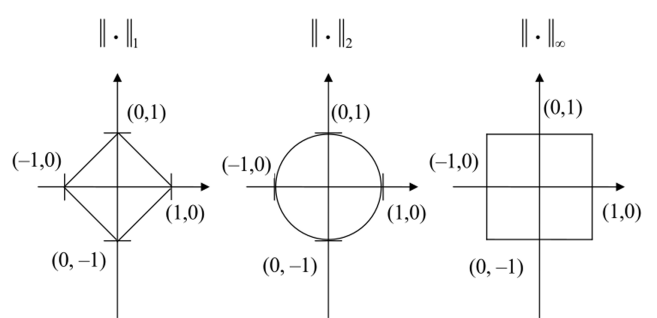
\includegraphics[width=0.7\textwidth]{pic1}
			\caption{нормы}
			\label{pic1}
		\end{figure}		
		
	\end{enumerate}
	
	
\end{document} 